\documentclass[../main.tex]{subfiles}

\begin{document}

In the previous section we described the algorithmic implementation of the 3D classification method. In this section we aim to explain how the code was structured to approach this task. Most of the code was developed as a Scipion protocol, although some specific tasks were delegated to separate programs.

\subsection{Scipion protocol}
Scipion is a \gls{cryoem} image processing platform that integrates many widespread image processing packages through plugins. Each plugin consists of a collection of programs known as protocols. Usually, protocols can be seen as high-level steps of an image processing pipeline. Indeed, a 3D classification can be considered as a protocol.

In this project, we have implemented our program as a Scipion protocol inside the Xmipp plugin. The protocol is named as \texttt{split volume} although this does not need to be confused with the old \texttt{split volume} protocol it replaces.

Typically, a Scipion protocol defines a set of input parameters which are displayed in the \gls{gui} when launching the protocol. The most relevant parameters of our protocol are listed hereafter:

\begin{itemize}
    \item \textbf{Input particles}: The particles analyzed during execution
    \item \textbf{Input mask (optional)}: A binary mask defining the \gls{roi} on which the classification focuses. If not provided, an spherical mask is automatically generated
    \item \textbf{Symmetry group}: If the protein under study exhibits a particular symmetry, this can be specified here to reduce projection directions.
    \item \textbf{Resize (optional)}: Controls if the particles are down sampled to a particular size. If not provided, particles are not resized.
    \item \textbf{Angular sampling}: Average spacing between angular groups. Defaults to 7.5 degrees.
\end{itemize}

Once the protocol is launched, it executes a series of operations known as steps. In the case of our protocol, these steps are linear, meaning that they are executed sequentially. The heavy operations are usually delegated to standalone programs, whilst the straightforward operations are implemented inside the protocol steps. The most relevant steps from our protocol are detailed here:

\begin{enumerate}
    \item \textbf{Convert input}: The input is converted to an appropriate format for our processing. If downsampling is selected, this downsampling occurs here.
    \item \textbf{Angular neighborhood}: Groups particles according to their projection directions. To do so, the existing \texttt{xmipp\_angular\_neighbourhood} program is used.
    \item \textbf{Classify directions step}: Each group is classified into two classes as dissimilar as possible. This is achieved with a newly created ad-hoc program named as\\ \texttt{xmipp\_aligned\_2d\_classification}, which will be detailed in the next section. 
    \item \textbf{Build graph}: Compares neighbouring classifications to build a graph with their similarities.
    \item \textbf{Graph optimization}: The maximum cut of the graph is computed so that classifications can be synchronized. \texttt{xmipp\_graph\_max\_cut} program was created to perform this task. 
    \item \textbf{Partition}: Once the classifications are synchronized, their log likelihood ratios are averaged and individual particles are classified according to their sign.
    \item \textbf{Reconstruction}: Each of the classes is used to produce a volume using the already existing \texttt{xmipp\_reconstruct\_fourier} program.
    \item \textbf{Create output}: Classes are converted to Scipion format.
\end{enumerate}

At the end, the Scipion protocol produces a set of classes and a set of volumes representing the classes. These objects may be used as input for another protocol that requires them, like for instance, a subsequent Relion 3D classification.

\subsection{Viewer}
Scipion protocol viewers are small \glspl{gui} that show detailed information about the protocol's execution. Therefore, a protocol viewer was also implemented for this algorithm for diagnose purposes. This viewer is able to present two visualizations related to its execution. 

Firstly, directions can be interactively analyzed to ensure that heterogeneity is being captured. To do so, a histogram of the \gls{pca} projection values is presented alongside the \gls{gmm} fitting. By dragging the yellow line, the user can visualize the heterogeneous state represented by the projection value. A snapshot of this representation is shown in Figure \ref{fig:4.2:classification_viewer}.

\begin{figure}[hbp]
    \centering
    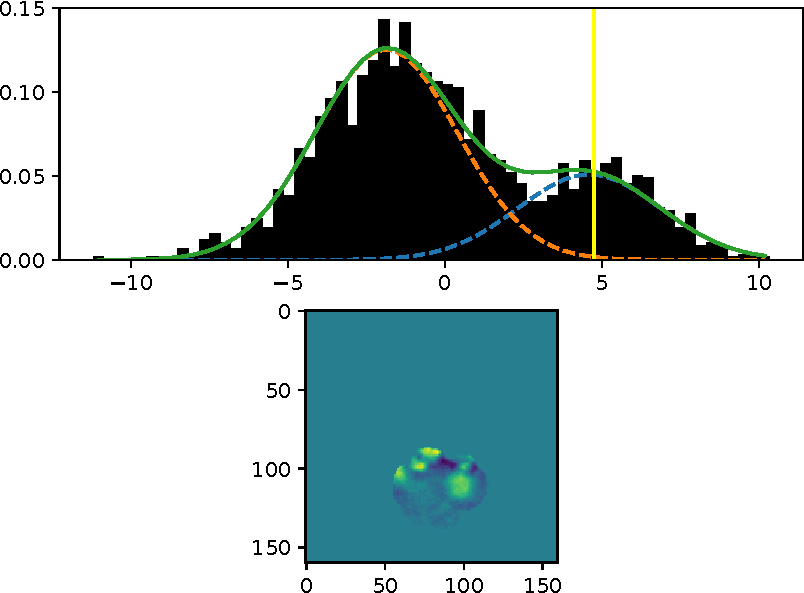
\includegraphics[width=.6\textwidth]{implementation/classification viewer}
    \caption{Snapshot of the classification viewer}
    \label{fig:4.2:classification_viewer}
\end{figure}

The other visualization involves a graph relating adjacent directions. This graph is embedded on a 3D sphere, which represents the projection directions. The edges of the graph are coloured so that they represent the weight attributed to it. This representation is displayed in Figure \ref{fig:4.2:graph_viewer}. Note that this graph is also interactive, the user may drag the cursor to change the viewing angle.

\begin{figure}[hbp]
    \centering
    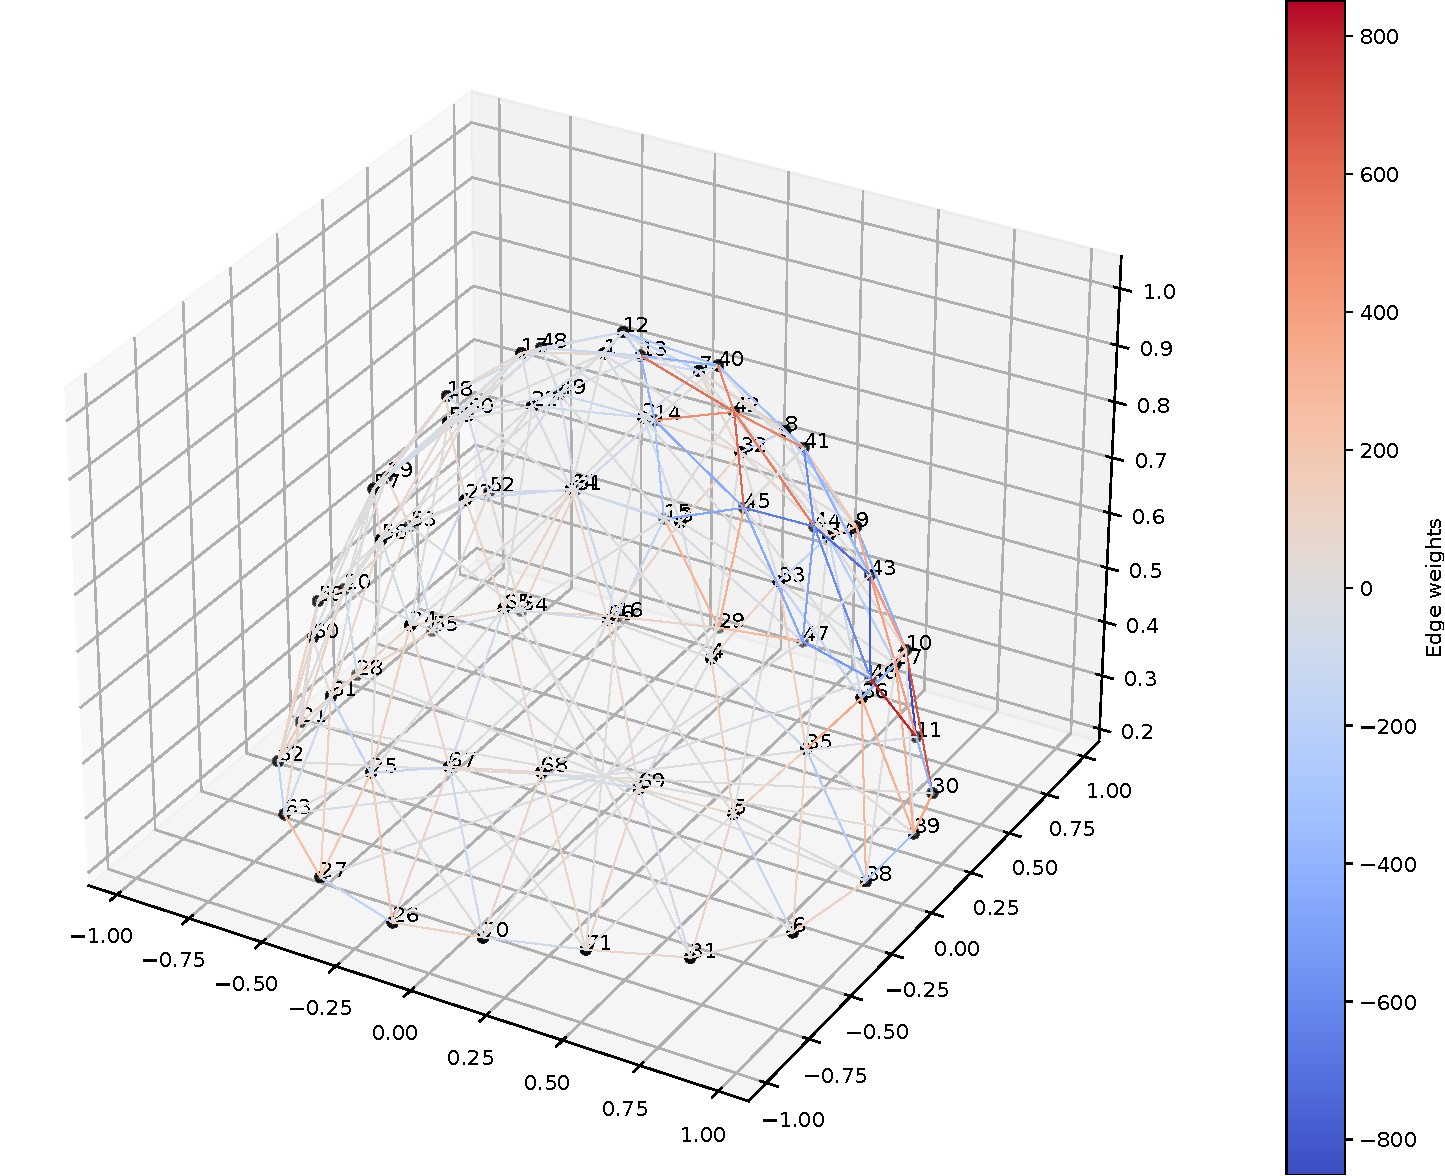
\includegraphics[width=.8\textwidth]{implementation/graph viewer}
    \caption{Snapshot of the 3D graph viewer}
    \label{fig:4.2:graph_viewer}
\end{figure}

\subsection{Auxiliary programs}
As mentioned earlier, computationally intensive operations were segregated from the protocol logic into their own programs. Then, these programs are invoked by the protocol. This separation benefits cluster users, as programs invoked by Scipion protocols can be dispatched to queue engines such as Slurm. In addition, it helps distinguishing the general control logic from the algorithmic nuances.

\subsubsection{Aligned 2D classification}
This program receives a set of images with their corresponding 3D alignment parameters and a reference direction. Then, it aligns the images to the reference projection direction and computes their \gls{pca}. These \gls{pca} projection values can be used to evaluate the class of each particle. We use \texttt{pytorch} to transform the images and compute the \gls{pca}.

Note that in our implementation we fit a \gls{gmm} model to these \gls{pca} projection values. This fitting is performed by the protocol itself and not the classification program. 

\subsubsection{Graph max cut}
Another computationally demanding task is the graph maximum cut. As mentioned in the previous section, we translate the maximum cut problem into a semi-definite programming program, which is solved by \texttt{cvxpy}. This program precisely does this translation. It takes a potentially sparse matrix representing the adjacency matrix of a graph and it converts it into a semi-definite programming problem. Once solved, it outputs a two sets of indices expressing the vertices corresponding to each of the partitions of the graph.

\end{document}
